
%!TEX program = xelatex

% Name           : demo.tex
% Author         : Moritz Flöter
% Version        : 1.0
% Created on     : 17.04.2016
% Last Edited on : 03.04.2017
% Copyright      : Copyright (c) 2016-2017 by Moritz Flöter.
% Based on       : HSRM-Theme from Benjamin Weiss
% License        : This file may be distributed and/or modified under the
%                  GNU Public License.
% Description    : HSRM beamer theme demonstration. Also includes a short 
%                  Tutorial regarding the beamer class.

%--------------------------------------------------------------------------
% aspectratio -> 4:3 -> 43, 16:9 -> 169, 16:10 -> 1610 etc.
%--------------------------------------------------------------------------
\documentclass[compress, aspectratio=43, noserifmath]{beamer}
%--------------------------------------------------------------------------
% Common packages
%--------------------------------------------------------------------------
\usepackage[german]{babel}
\usepackage[cache=false,outputdir=.texpadtmp]{minted}
\usepackage{graphicx}
\usepackage{multicol}
\usepackage{listingsutf8}
% Erweiterte Tabellenfunktionen
\usepackage{tabularx,ragged2e}
\usepackage{booktabs}
% Listingserweiterung
\usepackage{listings}
\lstset{ %
language=[LaTeX]TeX,
basicstyle=\normalsize\ttfamily,
keywordstyle=,
numbers=left,
numberstyle=\tiny\ttfamily,
stepnumber=1,
showspaces=false,
showstringspaces=false,
showtabs=false,
breaklines=true,
frame=tb,
framerule=0.5pt,
tabsize=4,
framexleftmargin=0.5em,
framexrightmargin=0.5em,
xleftmargin=0.5em,
xrightmargin=0.5em
}

%--------------------------------------------------------------------------
% Load theme
%--------------------------------------------------------------------------
\usetheme{freshroboto}


% must be loaded after theme
\usepackage{tikz}
\usetikzlibrary{mindmap,backgrounds}

%--------------------------------------------------------------------------
% General presentation settings
%--------------------------------------------------------------------------
\title{Prototypical Realization and Validation of an Incremental Software Product Line Analysis Approach}
\subtitle{Pr\"asentation zur Masterarbeit}
\date{Letztes Update: \today}
\author{Moritz Fl\"oter}
\institute{\textbf{Universit\"at Hildesheim}}

%--------------------------------------------------------------------------
% Notes settings
%--------------------------------------------------------------------------
\setbeameroption{show notes}

\begin{document}
%--------------------------------------------------------------------------
% Titlepage
%--------------------------------------------------------------------------

\maketitle

%\begin{frame}[plain]
%	\titlepage
%\end{frame}

%--------------------------------------------------------------------------
% Table of contents
%--------------------------------------------------------------------------
\section*{Gliederung}
\begin{frame}{Gliederung}
	% hideallsubsections ist empfehlenswert für längere Präsentationen
	\tableofcontents[hideallsubsections]

\end{frame}


\section{Idee \& Motivation}
\subsection{Idee \& Motivation}

\begin{frame}{Ist-Zustand}
\begin{itemize}
        \item[\textbullet] Analysen unterst\"utzen Softwareentwicklung
        \item[\textbullet] Analysen f\"ur Software Produktlinien (SPL) sind rechenintensiv
\end{itemize}
\end{frame}

\begin{frame}{Ist-Zustand}
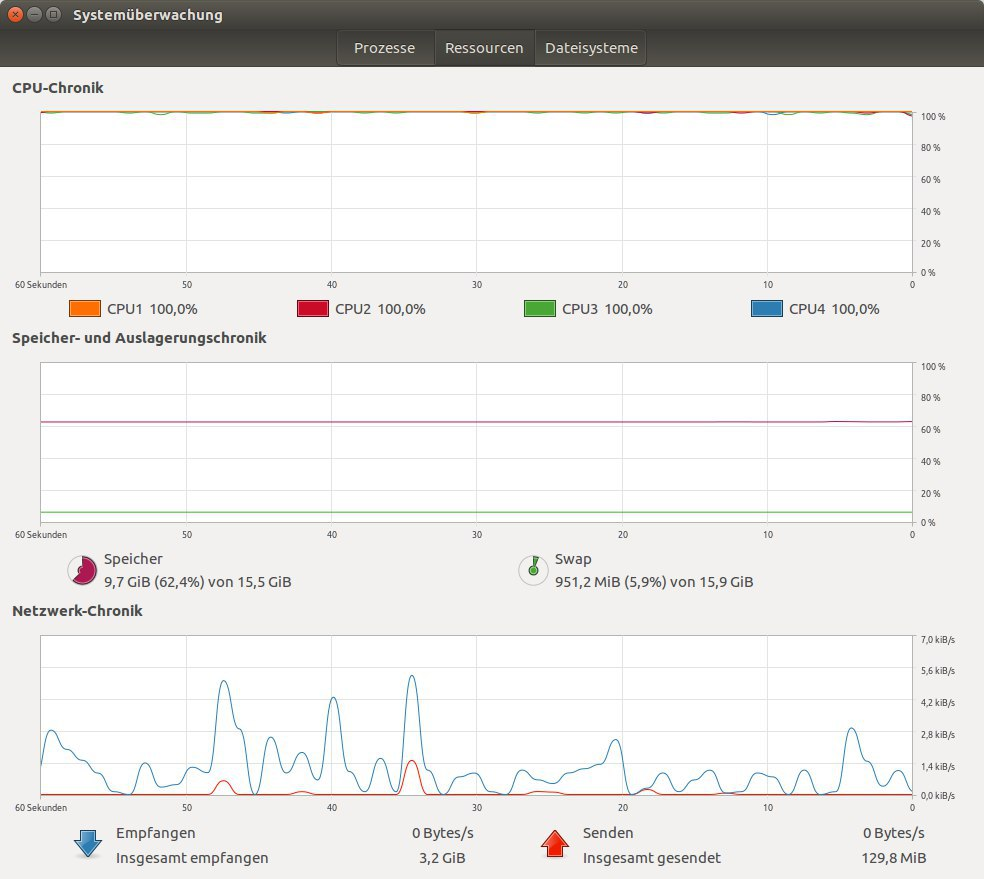
\includegraphics[width=1\textwidth]{image/cpu-analysis.jpg}
\end{frame}

\begin{frame}{Ist-Zustand}
\begin{itemize}
    \item[\textbullet] Relativ sp\"ate Verf\"ugbarkeit von Ergebnissen
    \item[\textbullet] Entwickler macht mittlerweile was anderes
\end{itemize}
\end{frame}

\begin{frame}{Idee}
Inkrementelle Analysen
\begin{itemize}
    \item[\textbullet] Nicht jedes mal alles neu analysieren
    \item[\textbullet] \"Uber eingef\"uhrte Ver\"anderungen bestimmen, welcher Teil analysiert werden muss 
\end{itemize}
\end{frame}



\section{Grundlagen}
\subsection{Grundlagen}

{ % all template changes are local to this group.
    \setbeamertemplate{navigation symbols}{}
    \begin{frame}[plain]
        \begin{tikzpicture}[remember picture,overlay]
            \node[at=(current page.center)] {
                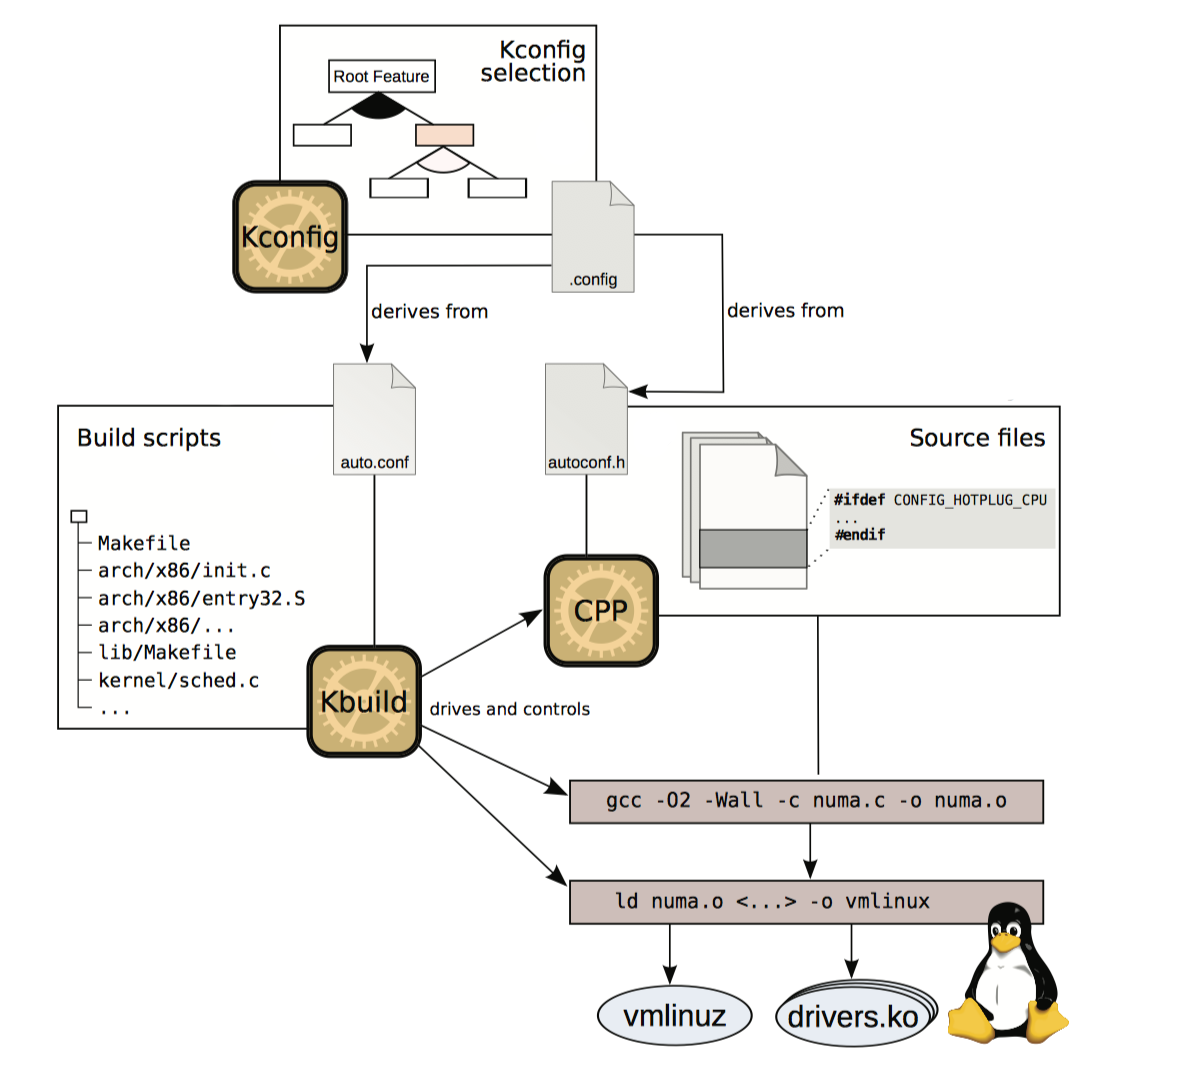
\includegraphics[width=1.0\textwidth]{image/linux-build2}
            };
        \end{tikzpicture}
     \end{frame}
}

\begin{frame}[containsverbatim]{Variabilit\"at - Variability Model}
\begin{minted}{kconfig}
config NETWORK_AUTHENTICATION
	bool "Network Authentication"
	depends on USER_AUTHENTICATION
	select NETWORK_SUPPORT
	default y
	help
	  Network authentication support ...

\end{minted}
\end{frame}


\begin{frame}[containsverbatim]{Variabilit\"at - Build Model}
\begin{minted}{make}
# Makefile for network device drivers.
obj-$(CONFIG_NETWORK_SUPPORT) += generic-driver.o
obj-$(CONFIG_NETWORK_SUPPORT) += other-drivers/

\end{minted}
\end{frame}



\begin{frame}[containsverbatim]{Variabilit\"at - Code Model}
   
\begin{minted}{cpp}
 #ifdef CONFIG_NETWORK_SUPPORT
   return 0;
 #else 
   return 1;
 #endif
\end{minted}
\end{frame}





\begin{frame}{KernelHaven}
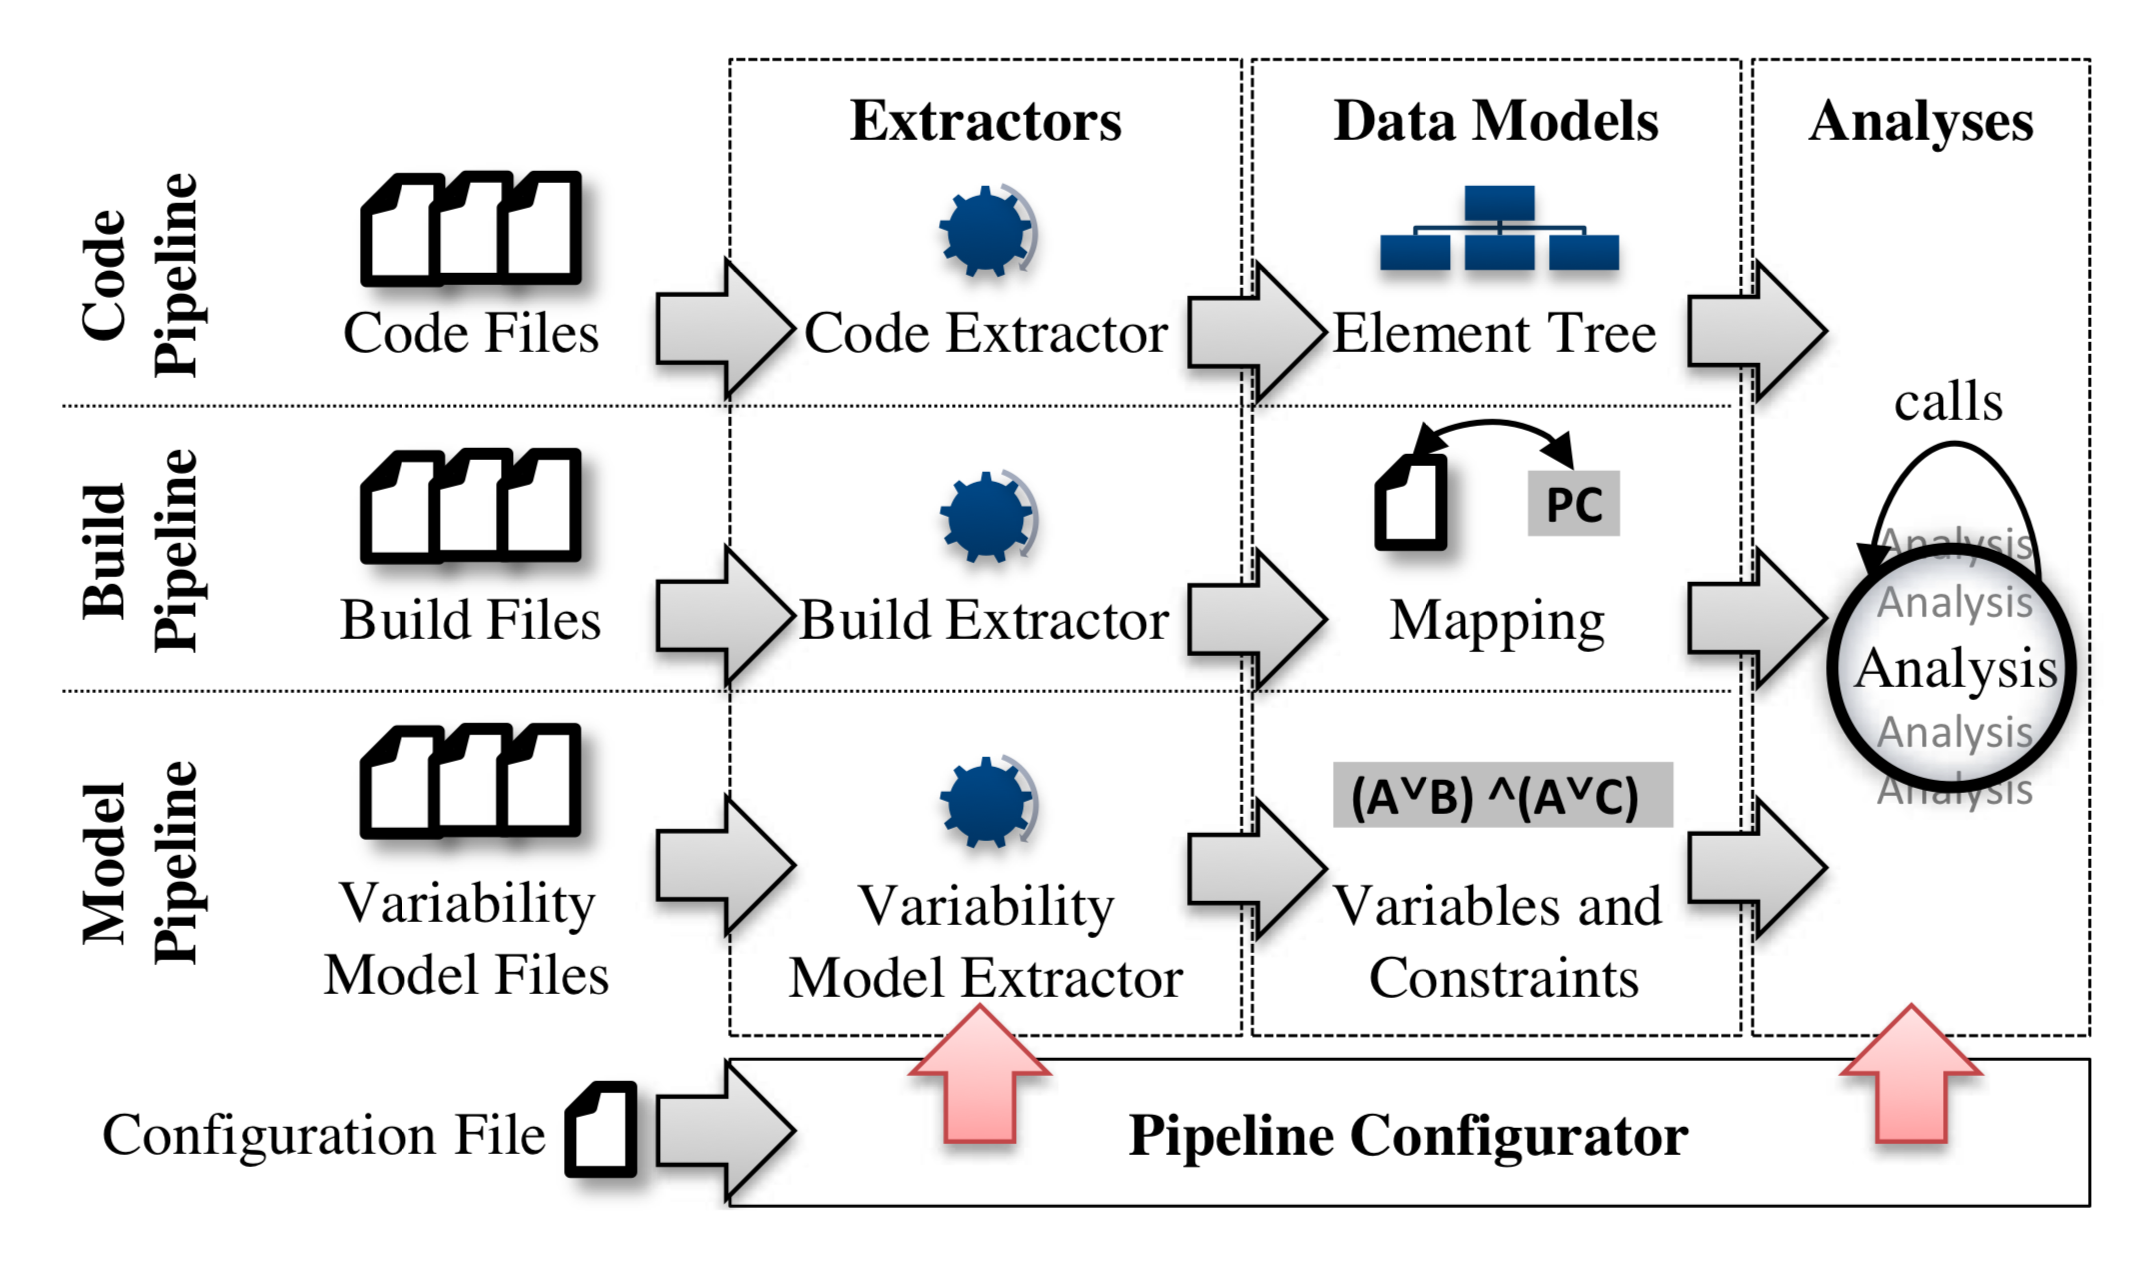
\includegraphics[width=1\textwidth]{image/KernelHaven-Pipeline}
\end{frame}

\begin{frame}[containsverbatim]{Dead Code Analyse - SPL}

\begin{minted}{python}
#ifdef CONFIG_NETWORK_AUTHENTICATION
  #ifdef !CONFIG_NETWORK_SUPPORT
    printf("You can not sign in");
  #endif
#endif
\end{minted}
\begin{minted}{kconfig}
config NETWORK_AUTHENTICATION
	bool "Network Authentication"
	...
	select NETWORK_SUPPORT
	...
\end{minted}
\end{frame}

\section{Konzept \& Implementierung}
\subsection{Konzept \& Implementierung}

\begin{frame}{Reduzierung des Aufwands}

Neu eingef\"uhrte Ver\"anderungen bestimmen, was erneut verarbeitet werden muss.
\begin{enumerate}
	\item Extraktion \\
	\emph{Die Extraktion der Modelle muss nicht vollst\"andig neu durchgef\"uhrt werden}
	\item Analyse \\
	\emph{Die Analyse muss nicht vollst\"andig neu durchgef\"uhrt werden}
\end{enumerate}
\end{frame}

\begin{frame}{Besondere Anforderungen}
F\"ur die Entwicklung wurden 14 Anforderungen festgelegt.
\begin{enumerate}
	\item Rollback \\
	\emph{}
	\item Analyse \\
	\emph{Die Analyse muss nicht vollst\"andig neu durchgef\"uhrt werden}
\end{enumerate}
\end{frame}



\begin{frame}{Nicht inkrementelle Analysen}
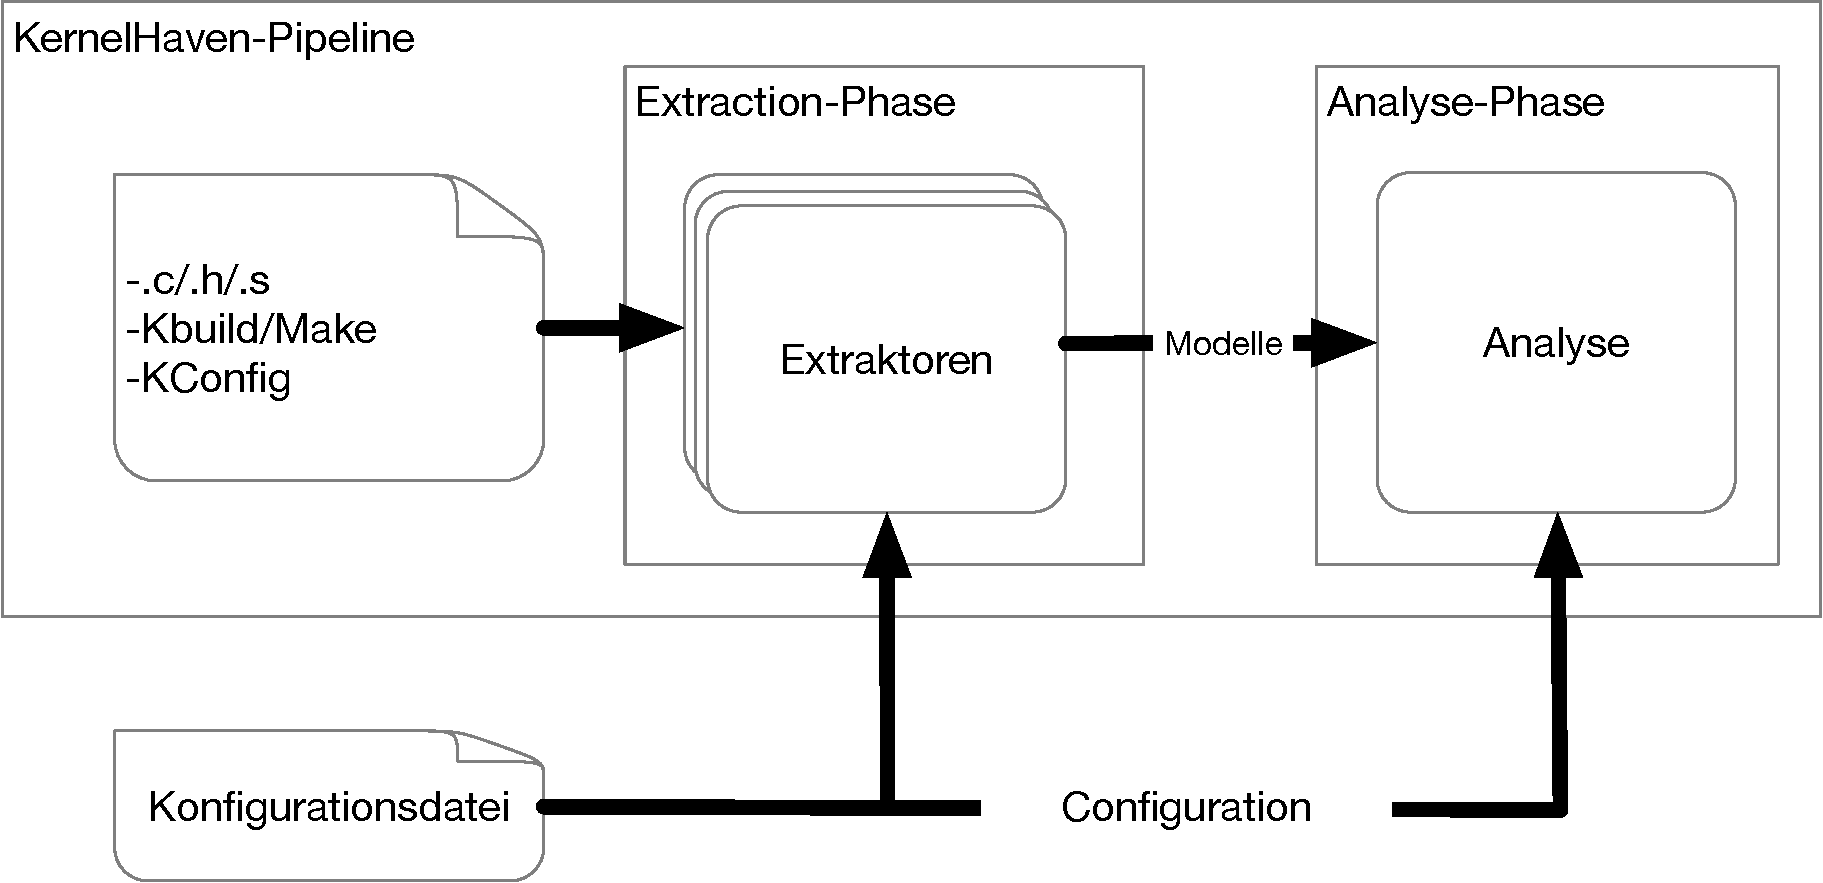
\includegraphics[width=1\textwidth]{image/KernelHaven.pdf}

\end{frame}


\begin{frame}{Inkrementelle Analysen}
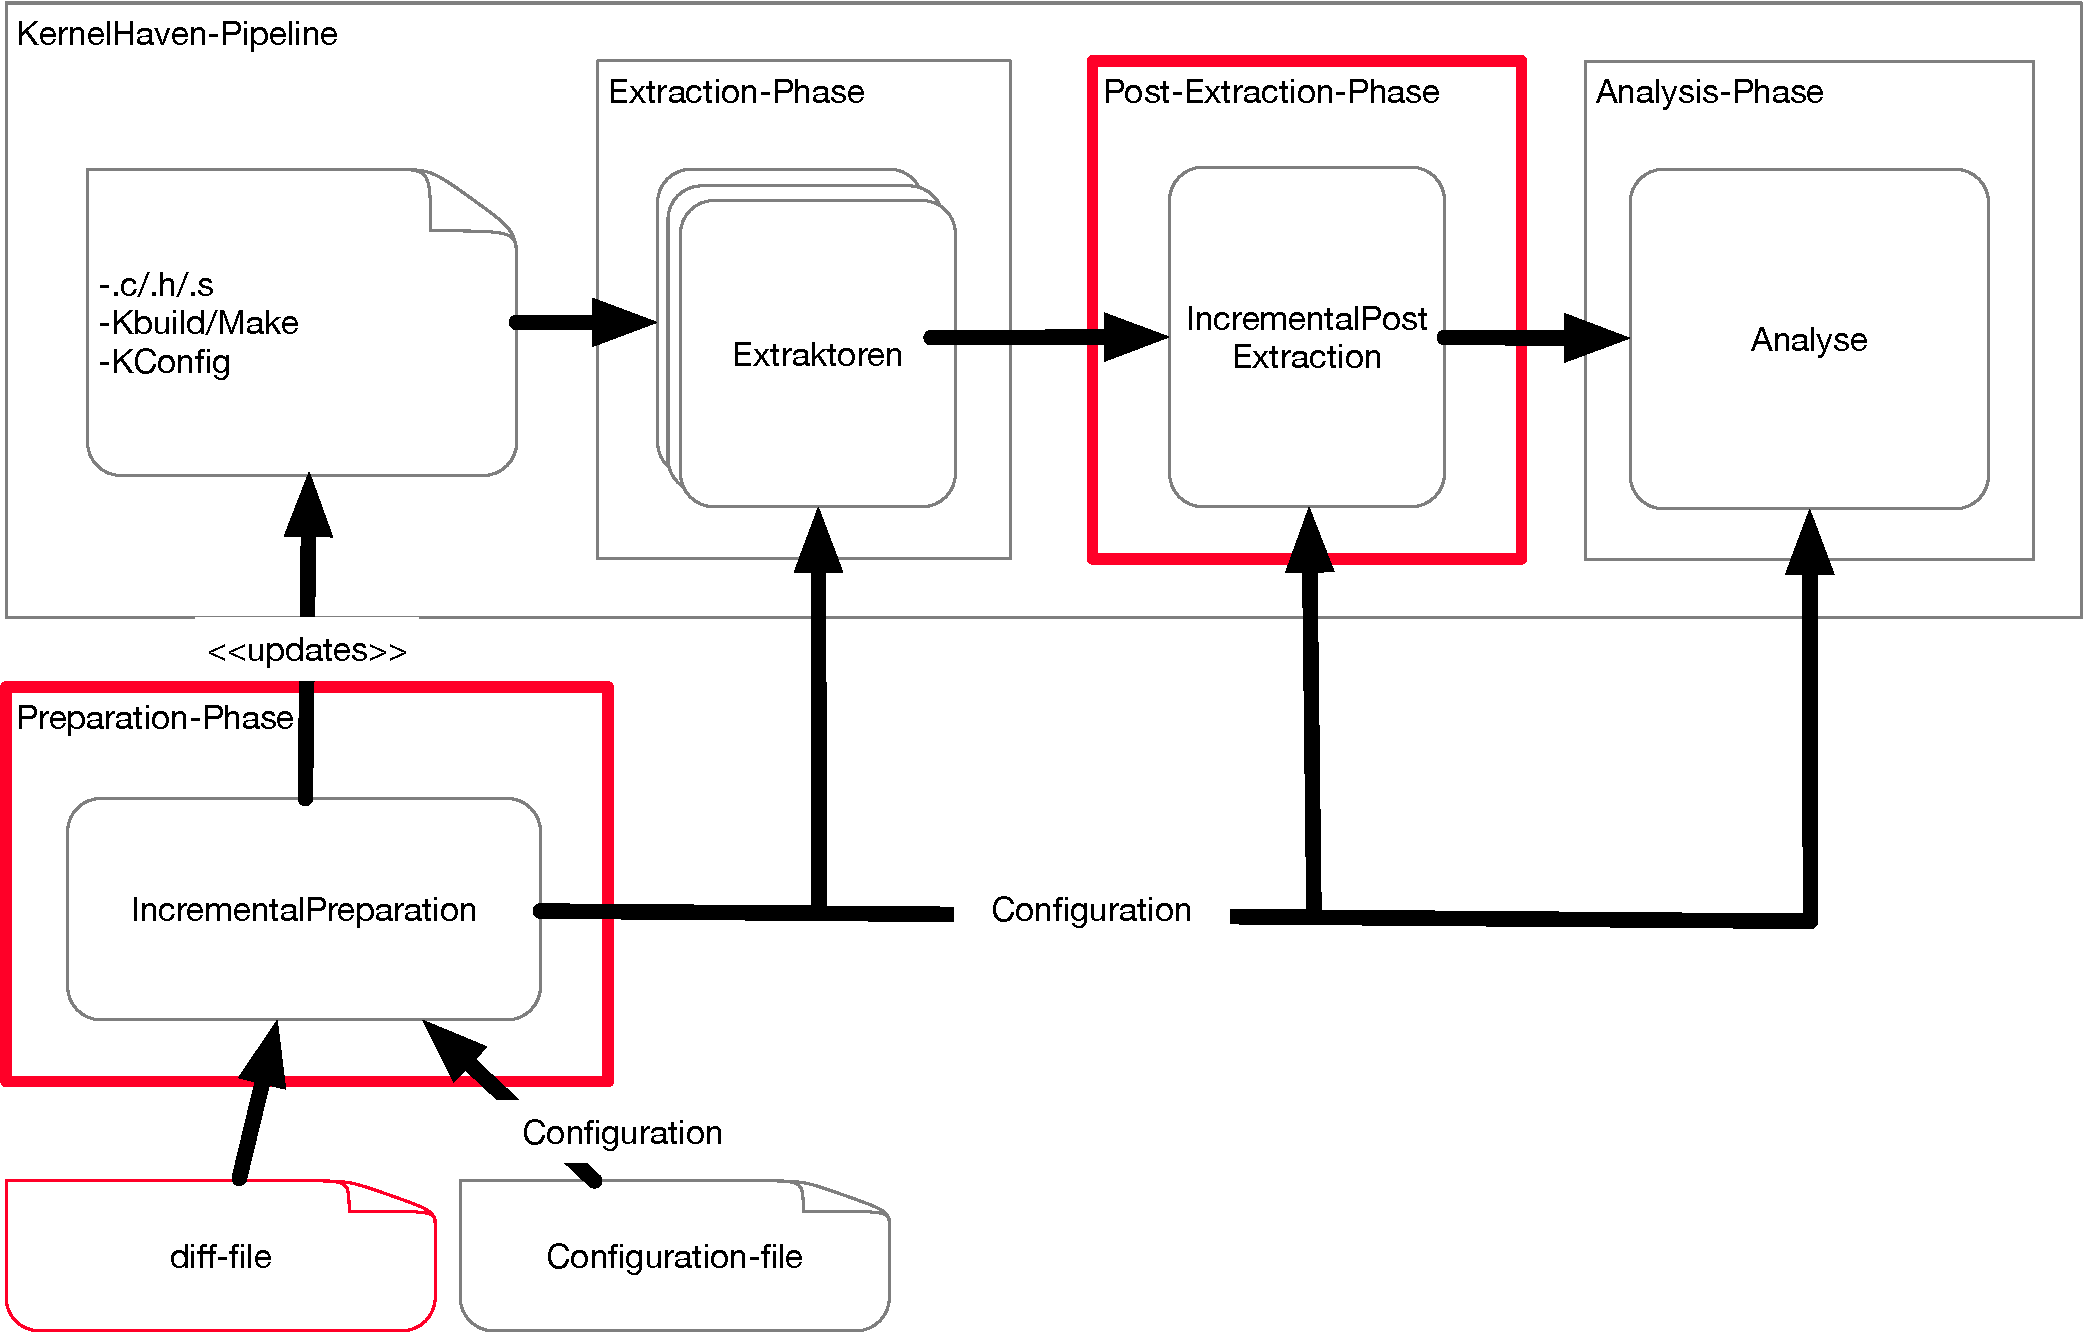
\includegraphics[width=1\textwidth]{image/KernelHavenIncremental.pdf}
\end{frame}


\begin{frame}{Preparation-Phase}
Aufgaben der Preparation-Phase
\begin{enumerate}
    \item Anwenden der \"Anderungen auf die Codebase
    \item Filtern von Dateien f\"ur Extraktion
    \item Anpassen der Konfiguration
\end{enumerate}
\end{frame}

\begin{frame}[containsverbatim]{Preparation-Phase}
1. Anwenden der \"Anderungen auf die Codebase

\begin{minted}{shell}
$ git apply path/to/git.diff
$ git apply --reverse path/to/git.diff
\end{minted}

\end{frame}


\begin{frame}{Post-Extraction-Phase}
Aufgaben der Post-Extraction-Phase
\begin{enumerate}
    \item Erhalt der Extraktions-Ergebnisse
    \item Zusammenf\"ugen mit vorigen Extraktions-Ergebnissen
\end{enumerate}
\end{frame}




\end{document}
